\documentclass[a4paper,11pt,uplatex]{jsarticle}
\usepackage[dvipdfmx]{graphicx}
\usepackage{url}

% タイトルと氏名
\title{日本におけるデジタル化の状況}
\author{G684622026 清水 一}
\date{2026年7月6日}

\begin{document}

\maketitle

\section{デジタル競争ランキング}
国際経営開発研究所(IMD)の調査\cite{imd}によると、日本のデジタル競争のランキングは図\ref{fig:ranking}に示すように、調査対象の64カ国中、総合で28位、知識分野で25位となっている。

\begin{figure}[htbp]
  \centering
  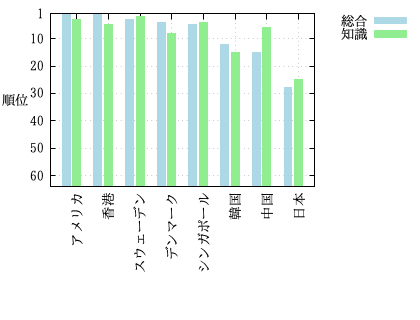
\includegraphics[width=0.8\linewidth]{fig31.png}
  \caption{デジタル競争ランキング(64カ国中)}
  \label{fig:ranking}
\end{figure}

\section{ブロードバンドの整備状況}
OECDによるブロードバンド回線の普及に関する調査\cite{oecd}によると、表\ref{tab:broadband}に示すように、日本における100人あたりのモバイルブロードバンドの加入者数は190.5で、第1位になっている。2位はエストニアで、3位米国と続く。

\begin{table}[htbp]
  \centering
  \caption{モバイルブロードバンドの加入者数(100人あたり)}
  \label{tab:broadband}
  \begin{tabular}{|l|l|l|}
    \hline
    順位 & 国名 & 加入者数 \\ \hline
    1位 & 日本 & 190.5 \\ \hline
    2位 & エストニア & 179.9 \\ \hline
    3位 & 米国 & 169.0 \\ \hline
    4位 & フィンランド & 157.0 \\ \hline
    5位 & デンマーク & 141.7 \\ \hline
    6位 & ラトビア & 141.6 \\ \hline
    7位 & イスラエル & 139.9 \\ \hline
    8位 & オランダ & 133.7 \\ \hline
    9位 & ポーランド & 131.3 \\ \hline
    10位 & スウェーデン & 127.2 \\ \hline
  \end{tabular}
\end{table}

\section{考察}
以上の調査結果について、自分が考えたことをここに記述すること。
\begin{itemize}
    \item 通信インフラの普及率が世界１位であるのに対し、デジタル競争ランキングは28位と低迷している
    \item デジタル競争ランキングの低さは、デジタル技術の活用やイノベーションの促進において課題があることを示している可能性がある
\end{itemize}

\bibliographystyle{junsrt}
\bibliography{exercise}

\end{document}
